The \acronymMGRAO{}{} algorithm helps agents executing atomic tasks allocate their resources to optimise the corresponding composite task value. 
\begin{figure}[ht]
	\centering
	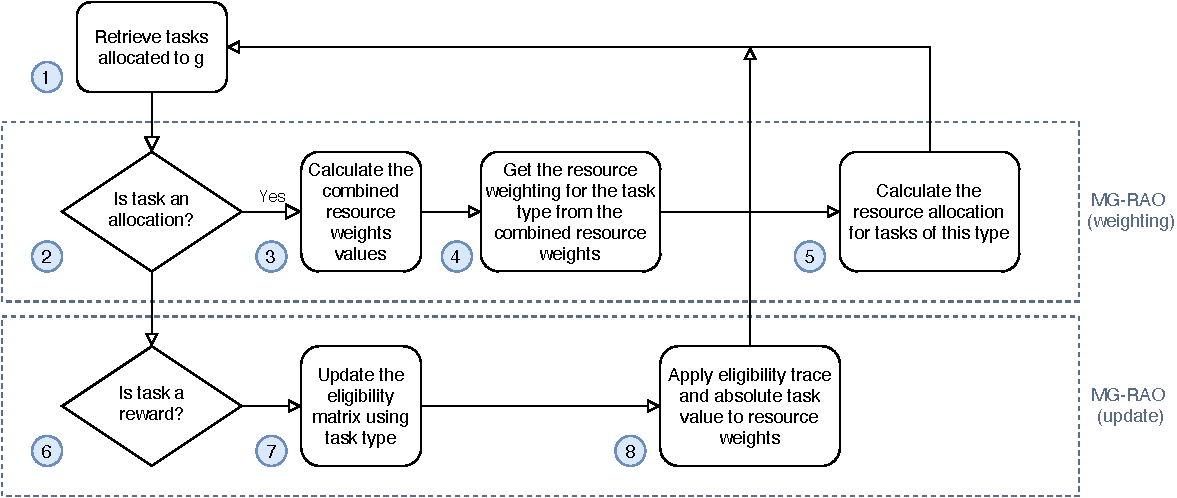
\includegraphics[width=0.8\linewidth, trim={55pt 0pt 55pt 0pt, clip}]{mgrao-simplified}
	\caption{\textbf{Simplified \acronymMGRAO{}{} flowchart}. The diagram shows the decision-making and actions taken by an agent using the \acronymMGRAO{}{}  algorithm. This is a combination of two sub-algorithms, \acronymMGRAO{}{}(weighting), that returns the amount of the agents resources that are allocated to completing the requested task type, and  \acronymMGRAO{}{}(update), that updates its resource weightings from rewards for previous atomic task completions. \newline
		\textbf{(1)} The agent processes its current tasks. \newline
		\textbf{(2-5)} If the task is a request for information, the agent will randomly select knowledge of other system agents from its knowledge base and return this information to the requester. \newline
		\textbf{(6-8)} If the task is a reward for a previously completed task, the agent will update its eligibility matrix using the task type, allowing the reward for task to be spread across a number of previous past actions. It will then use the absolute task value that is sent as part of the reward task, to attempt optimisation of its resource allocation by adjusting their balance across possible task types.  \newline
	}
	\label{fig:mgrao-simplified}
\end{figure}

This has two parts, an update algorithm that adjusts weights of resources based on received atomic task values, $\label{eq:mgrao_update}\formalMGRAOUpdate{}{}$,  and the application of these weights to generate the task execution quality itself, $\label{eq:mgrao_weighting}\formalMGRAOWeighting{}{}$. The update algorithm will change the resource weightings for an agent, $\functionAgentResources{}{}$, given the type of an atomic task completed, and the its absolute task value to the corresponding composite task. The weighting algorithm simply returns the resource weighting for calculation of an atomic tasks' quality $\functionAtomicTaskQualitySignature{}{}$ on its completion.